\documentclass{article}\usepackage[]{graphicx}\usepackage[]{color}
%% maxwidth is the original width if it is less than linewidth
%% otherwise use linewidth (to make sure the graphics do not exceed the margin)
\makeatletter
\def\maxwidth{ %
  \ifdim\Gin@nat@width>\linewidth
    \linewidth
  \else
    \Gin@nat@width
  \fi
}
\makeatother

\definecolor{fgcolor}{rgb}{0.345, 0.345, 0.345}
\newcommand{\hlnum}[1]{\textcolor[rgb]{0.686,0.059,0.569}{#1}}%
\newcommand{\hlstr}[1]{\textcolor[rgb]{0.192,0.494,0.8}{#1}}%
\newcommand{\hlcom}[1]{\textcolor[rgb]{0.678,0.584,0.686}{\textit{#1}}}%
\newcommand{\hlopt}[1]{\textcolor[rgb]{0,0,0}{#1}}%
\newcommand{\hlstd}[1]{\textcolor[rgb]{0.345,0.345,0.345}{#1}}%
\newcommand{\hlkwa}[1]{\textcolor[rgb]{0.161,0.373,0.58}{\textbf{#1}}}%
\newcommand{\hlkwb}[1]{\textcolor[rgb]{0.69,0.353,0.396}{#1}}%
\newcommand{\hlkwc}[1]{\textcolor[rgb]{0.333,0.667,0.333}{#1}}%
\newcommand{\hlkwd}[1]{\textcolor[rgb]{0.737,0.353,0.396}{\textbf{#1}}}%

\usepackage{framed}
\makeatletter
\newenvironment{kframe}{%
 \def\at@end@of@kframe{}%
 \ifinner\ifhmode%
  \def\at@end@of@kframe{\end{minipage}}%
  \begin{minipage}{\columnwidth}%
 \fi\fi%
 \def\FrameCommand##1{\hskip\@totalleftmargin \hskip-\fboxsep
 \colorbox{shadecolor}{##1}\hskip-\fboxsep
     % There is no \\@totalrightmargin, so:
     \hskip-\linewidth \hskip-\@totalleftmargin \hskip\columnwidth}%
 \MakeFramed {\advance\hsize-\width
   \@totalleftmargin\z@ \linewidth\hsize
   \@setminipage}}%
 {\par\unskip\endMakeFramed%
 \at@end@of@kframe}
\makeatother

\definecolor{shadecolor}{rgb}{.97, .97, .97}
\definecolor{messagecolor}{rgb}{0, 0, 0}
\definecolor{warningcolor}{rgb}{1, 0, 1}
\definecolor{errorcolor}{rgb}{1, 0, 0}
\newenvironment{knitrout}{}{} % an empty environment to be redefined in TeX

\usepackage{alltt}
\usepackage{Sweave}
\usepackage{float}
\usepackage{graphicx}
\usepackage{tabularx}
\usepackage{siunitx}
\usepackage{mdframed}
\usepackage{natbib}
\bibliographystyle{..//refs/styles/besjournals.bst}
\usepackage[small]{caption}
\setkeys{Gin}{width=0.8\textwidth}
\setlength{\captionmargin}{30pt}
\setlength{\abovecaptionskip}{0pt}
\setlength{\belowcaptionskip}{10pt}
\topmargin -1.5cm        
\oddsidemargin -0.04cm   
\evensidemargin -0.04cm
\textwidth 16.59cm
\textheight 21.94cm 
%\pagestyle{empty} %comment if want page numbers
\parskip 7.2pt
\renewcommand{\baselinestretch}{1.5}
\parindent 0pt

\newmdenv[
  topline=true,
  bottomline=true,
  skipabove=\topsep,
  skipbelow=\topsep
]{siderules}

%% R Script


\IfFileExists{upquote.sty}{\usepackage{upquote}}{}
\begin{document}
\title{Rethinking False Spring Risk}
\author{Chamberlain, Wolkovich}
\date{\today}
\maketitle 

\renewcommand{\thetable}{\arabic{table}}
\renewcommand{\thefigure}{\arabic{figure}}
\renewcommand{\labelitemi}{$-$}

%%%%%%%%%%%%%%%%%%%%%%%%%%%%%%%%%%%%%%%%%%%%%%%
\begin{center}
\LARGE\textbf{Outline}
\end{center}
\section{Introduction}
Plants growing in temperate environments are at risk of being exposed to late spring freezes, which can be detrimental to growth. Individuals that leaf out before the last frost are at risk of damaging wood tissue, leaf loss, and slowed or stalled canopy development \citep{Gu2008, Hufkens2012}. Therefore, temperate deciduous tree species must have plastic phenological responses in the spring in order to optimize photosynthesis and minimize frost or drought risk \citep{Polgar2011}. These late spring freezing events are known as false springs. False spring events can result in highly adverse ecological and economic consequences \citep{Ault2013, Knudson2012}.

Climate change is expected to increase damage from false spring events around the world due to earlier spring onset and greater fluctuations in temperature \citep{Martin2010, Inouye2008, Cannell1986}. Temperate forest species around the world are initiating leaf out about 4.6 days earlier per degree Celsius \citep{Polgar2014, Wolkovich2012}. It is anticipated that there will be a decrease in false spring frequency overall but the magnitude of temperature variation is likely to increase, therefore amplifying the expected intensity of false spring events \citep{Allstadt2015, Kodra2011}. Mulitple studies have documented false spring events in recent years \citep{Augspurger2013, Knudson2012, Augspurger2009, Gu2008} and some have linked this to climate change \citep{Muffler2016, Xin2016, Allstadt2015, Ault2013}. Due to these reasons, it is crucial for researchers to properly evaluate the effects of false spring events on temperate forests and agricultural crops in order to make more accurate predictions on future trends.

Different species respond differently to late spring freezing events. The level of damage sustained by plants from a false spring also varies across phenophases. Various studies have assessed the risk of damage or the intensity of particular false spring events but at this time false spring studies fail to incorporate all potential factors that could affect the level of frost damage risk. A False Spring Index (FSI) signifies the likelihood of a damage to occur from a late spring freeze. Currently, FSI evaluates day of budburst, number of growing degree days, and day of last spring freeze through a simple equation as seen below \citep{Marino2011}. 

\[ FSI = Julian Date (Last Spring Freeze) - Julian Date (Budburst) \]

If FSI is a positive number and greater than 7, then crown dieback is more likely to occur. False spring studies largely simplify the various ecological elements that could predict the level of plant damage from late spring freezing events. In contrast to these simplifications, we argue that a wealth of factors greatly impacts plants' frost spring risk such that simple indices will most likely lead to inaccurate predictions and ultimately do little to advance the field. 

In this paper we aim to highlight the complexity of factors driving a plant's false spring risk. We outline in particular how life stage of the individual \citep{Caffarra2011}, location within a forest or canopy \citep{Augspurger2013}, winter chilling hours (Flynn \& Wolkovich 2017?), proximity to water \citep{Gu2008}, level of precipitation prior to the freezing event \citep{Anderegg2013}, freeze duration/intensity, and range limits of the species \citep{Martin2010} unhinge simple metrics of false spring. The ultimate intent is to demonstrate how an integrated view of false spring that incorporates these factors would rapidly advance progress in this field.  

\section{Defining False Spring}
There are two phases involved in late spring freezing: rapid vegetative growth prior to the freeze and the post freeze setback. This combined process is known as a false spring \citep{Gu2008}. Freeze and thaw fluctuations can cause xylem embolism and decreased xylem conductivity which can result in crown dieback \citep{Gu2008}.

Warm temperatures earlier in the year (i.e. in February) do not seem to affect species, most likely because it is too soon for budburst to initiate and sufficient chilling has not yet occurred. Frost damage usually occurs when there is a warmer than average March, a freezing April, and enough growing days between the high temperatures and the last freeze date \citep{Augspurger2013}. 
FSI is considered significant if it is greater than 7 days between budburst and leafout \citep{Peterson2014}. The 7 day parameter exposes less resistant foliate phenophases to a freezing event and puts the plant at a higher risk of damage. There is much debate over the definition of freezing temperatures, which has resulted in two types of freezes: a ``hard'' freeze at -2.2$^{\circ}$C and a "soft" freeze at -1.7$^{\circ}$C \citep{Augspurger2013, Kodra2011, Vavrus2006}.

Once budburst has initiated, buds cannot respond to cold temperatures and freezing resistance is greatly reduced \citep{Vitasse2014, Lenz2013, Taschler2004}.

Freezing damage can occur directly via intracellular ice formation or indirectly via freezing dehydration \citep{Hofmann2015, Beck2004, Pearce2001}. Dry winters typically result in growth of new shoots with decreased water content which increases frost resistance because the osmotic potential within the shoots has decreased from accumulating solutes \citep{Hofmann2015, Morin2007}. Therefore, increased bud dehyration results in increased frost hardiness \citep{Hofmann2015, Kathke2011, Poirier2010, Nielsen2009, Beck2007}.

\subsection*{Determining Spring Onset}
Lizzie: "I think 'Determining Spring Onset' can go here but you need to develop idea first (e.g. canopy vs understory, species vs mix etc...) then results only and digest what they mean for reader.

Our projections indicate that observational FSI values are highly comparable to the USA-NPN FSI values, rendering both justifiable methods for determining potential risk involved in late spring freezes. Even though budburst is defined differently between Dr. O'Keefe, USA-NPN, and the PhenoCam, the dates of budburst are similar. The spring onset dates gathered from the PhenoCam dataset are different from the other two methods, which is likely due to fact that the PhenoCam data is assessing budburst for the forest canopy. Through the use of USA-NPN data, researchers could gather dates of budburst across multiple locations at once in order to determine False Spring risk, making it a more effective method than observational data. Although, all three methods are viable. Various studies have shown that understory species will initiate budburst earlier in the season in order to exploit open canopies and early growth, whereas late successional species may start later in the season to avoid frost or drought risk \citep{Xin2016, Richardson2009}. Therefore, the methodology used for determining spring onset should largely be dependent on the functional group of interest: researchers should use the USA-NPN dataset for understory species, PhenoCam data for late successional species, and observational data for a wide array of plant functional types. 

\begin{figure}[H]
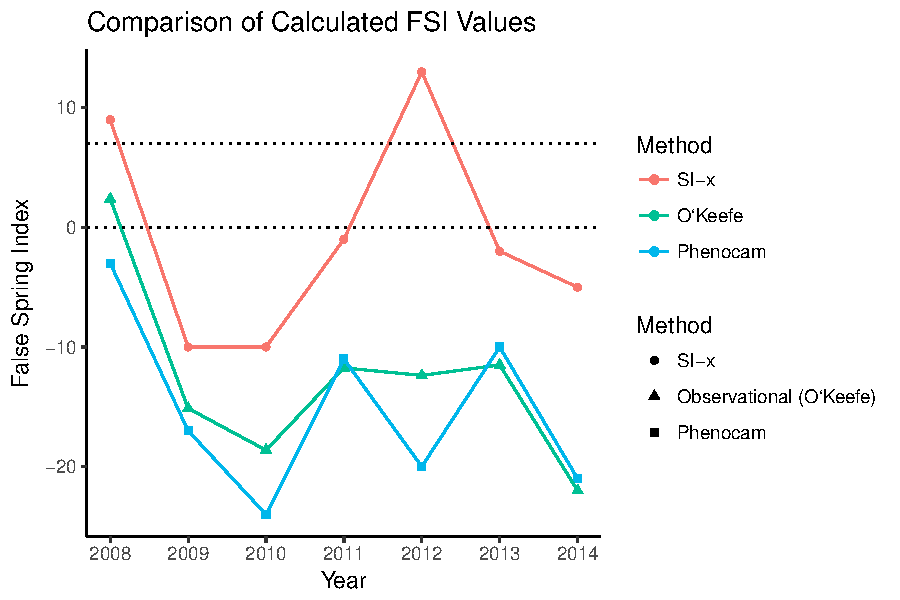
\includegraphics[width=\maxwidth]{figure/fsifig-1} \caption[A scatterplot indicating FSI values from 2008 to 2014 for each methdology used in this study]{A scatterplot indicating FSI values from 2008 to 2014 for each methdology used in this study. PhenoCam FSI values are red, Observed FSI values are blue, and USA-NPN FSI values are green.}\label{fig:fsifig}
\end{figure}



\section*{Understanding (Defining?) Vegetative Risk}
Lizzie: "Phenophases, Species differences (maybe just set up here...), regional differences?, some of your points in Box 1 here - basically set up everything that could matter then make a case for what matters most and hit on those in next sections."

Another highly crucial factor to consider is the rate of budburst and the length of time between budburst to full leafout, which we will refer to as the duration of vegetative risk.

\subsection*{Phenophases}
Spring frosts during the vegetative growth phenophases impose the greatest freezing threat to deciduous tree species \citep{Sakai1987}.

The level of damage sustained by plants from a false spring also varies across phenophases. Generally, reproductive phases are more sensitive to false spring events than vegetative phases and developing leaves are more susceptible to damage than opening buds or expanding shoots \citep{Lenz2013,Augspurger2009}. However, trees that suffer severe vegetative growth damage from a false spring event will suffer greater long-term effects from the loss of photosynthetic tissue than trees that lose one year of reproductive growth.

Phenophase is a greater indicator for level of risk than life stage. Inidivudals exhibiting a certain phenophase (i.e. between budburst and full leafout) are more likely to incur damage from a freezing event than individuals past the leafout phenophase, independent of life stage \citep{Augspurger2009,Vitasse2014}.

We will use the BBCH Scale Phase 09 to define budburst and Phase 15 to define leaf out \citep{Meier2001}.


\subsection*{Species}
Seedling and sapling individuals of canopy species initiate budburst before to canopy closure in order to benefit from the increased light levels \citep{Augspurger2008}, therefore putting them at greater risk to false spring damage than adult trees \citep{Vitasse2014}. Younger trees are more likely to incur lastly damage to the leaf buds and vegetative growth, whereas adult trees are at risk of xylem embolism. In order for xylem embolism to occur, extreme cavitation must first occur. Extensive cavitation in the xylem would require more intensive freezing events than it would take to damage seedling and sapling leaf buds. Especially strong freezing events (i.e. >-8.6$^{\circ}$C), could result in meristemic tissue, wood parenchyma and phloem damage \citep{Lenz2013, Augspurger2011, Sakai1987}.  

However, different species respond differently to anthropogenic climate change. Most species are expected to begin leaf out earlier in the season with warming spring temperatures but some species may have the opposite response \citep{Xin2016, Cleland2006, Yu2010}.

Studies indicate that species growing at more northern latitudes tend to respond greater to photoperiod than species growing further south \citep{Caffarra2011}. Similarly, late successional species exhibit greater photoperiod sensitivities than pioneer species \citep{Basler2012}. 

\section*{Species Differences and Vegetative Risk}
Lizzie: "You have so much great stuff here but need to develop WHY and HOW species would differ. You touch on this once in paper but need to develop more. This section should start with building a case for why species would differ then go into data."

Plants are most susceptible to frost damage between budburst and leafout \citep{Lenz2016, Vitasse2014, Augspurger2009}. The rate of budburst and the length of time between budburst and leafout is a crucial indicator for predicting level of damage from a false spring event. We will refer to the timing of these collective phenophases (i.e. budburst to leafout) as the duration of vegetative risk. The duration of vegetative risk increases if a freezing event occurs during the phenophases between budburst and leaf expansion and species with short durations of vegetative risk sustained higher levels of damage. Therefore, if the duration of vegetative risk is longer, then the buds and leaves will be heartier against frosts \citep{Augspurger2009}. Frost tolerance, however, steadily decreases after budburst begins until the leaf is fully unfolded, with leafout being the most susceptible to frost damage \citep{Lenz2016}. It is therefore crucial that more studies investigate the relationship between false spring events and duration of vegetative risk. 

\subsection*{Treespotters Data}

\begin{figure}[H]
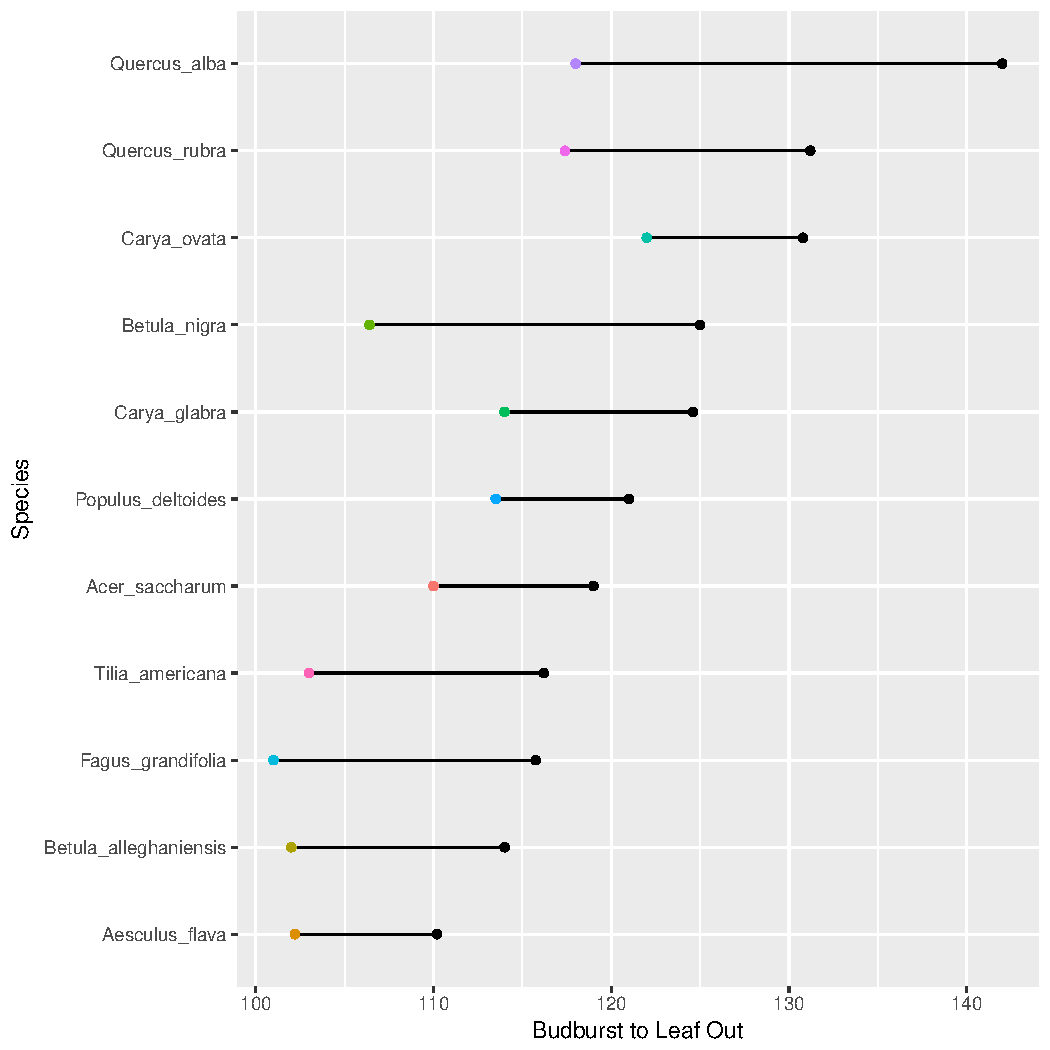
\includegraphics[width=\maxwidth]{figure/treespotters-1} \caption[A timeline plot indicating the duration of vegetative risk for each species studied at the Arnold Arboretum in 2016]{A timeline plot indicating the duration of vegetative risk for each species studied at the Arnold Arboretum in 2016.}\label{fig:treespotters}
\end{figure}



\subsection*{Dan's Data}
It is possible, that with anthropogenic climate change progressing, leaf out timing may be delayed. As winter seasons begin to warm and chilling requirements are not met, more warming in the spring must first occur for budburst to begin \citep{Polgar2014, Fu2012, Morin2009, McCreary1990}. In a chilling experiment performed by Flynn \& Wolkovich (2017), there were various experimental chilling, photoperiod, and forcing treatments. In Figure 2, five species were assessed across five different treatments. C is a forcing temperature of 15$^{\circ}$C during the day and 5$^{\circ}$C at night, W is a forcing temperature of 20$^{\circ}$C during the day and 10$^{\circ}$C at night, S is a short day with 8 hours of daylight, L is a long day with 12 hours of daylight, 0 is no additional winter chilling, 1 is 33 days of additional winter chilling at 4$^{\circ}$C, and 2 is 33 days of additional winter chilling at 1.5$^{\circ}$C. QUERUB is \textit{Quercus rubra}, ACERUB is \textit{Acer rubrum}, POPGRA is \textit{Populus grandidentata}, ILEMUC is \textit{Ilex mucronata}, BETPAP is \textit{Betula papyrifera}.

\begin{figure}[H]
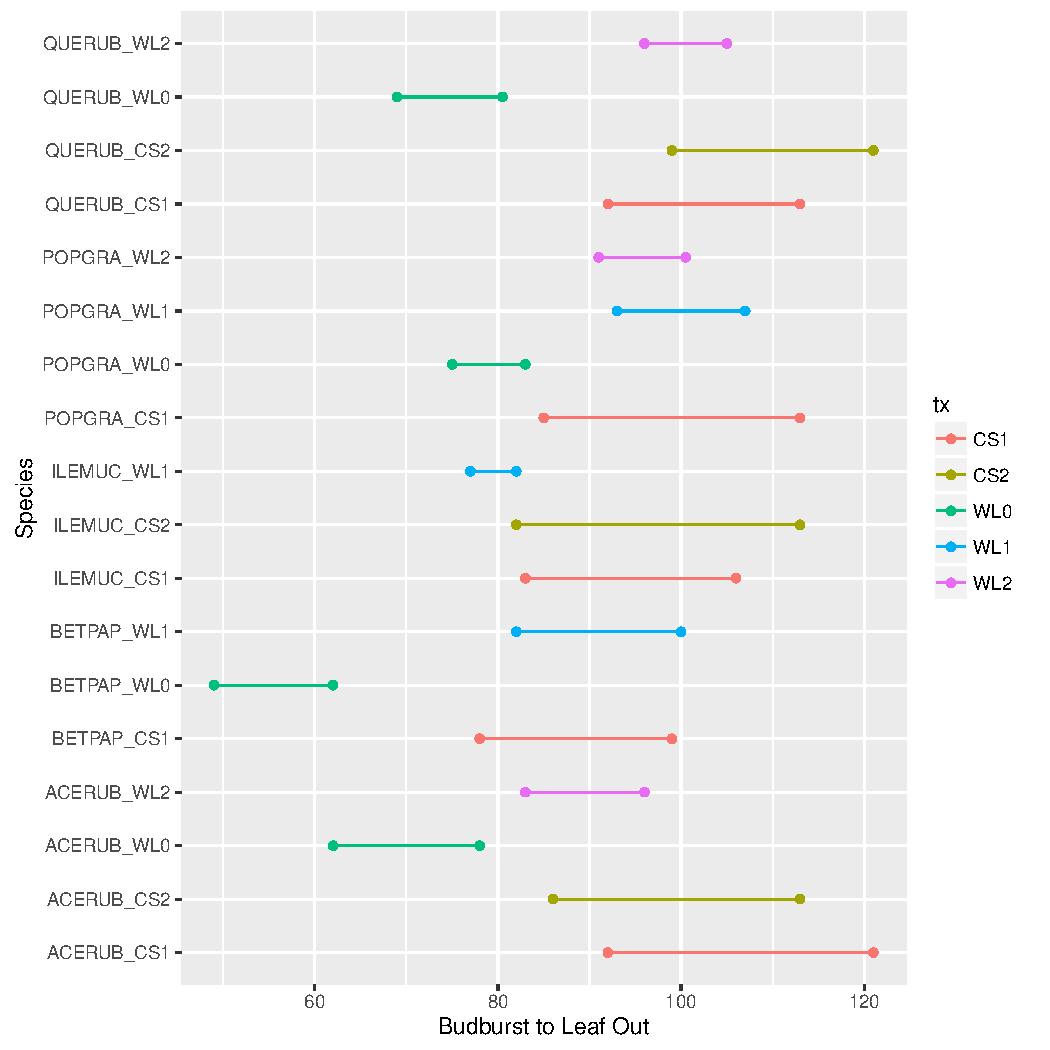
\includegraphics[width=\maxwidth]{figure/chilling-1} \caption[A timeline plot indicating the duration of vegetative risk for each species from experimental chilling study]{A timeline plot indicating the duration of vegetative risk for each species from experimental chilling study.}\label{fig:chilling}
\end{figure}





% Table created by stargazer v.5.2 by Marek Hlavac, Harvard University. E-mail: hlavac at fas.harvard.edu
% Date and time: Tue, Jan 24, 2017 - 10:22:38
\begin{table}[!htbp] \centering 
  \caption{The results from a linear regression model analyzing the relationship between duration of vegetation risk and intial budburst across five treatments} 
  \label{} 
\begin{tabular}{@{\extracolsep{5pt}}lc} 
\\[-1.8ex]\hline 
\hline \\[-1.8ex] 
 & \multicolumn{1}{c}{\textit{Dependent variable:}} \\ 
\cline{2-2} 
\\[-1.8ex] & Risk \\ 
\hline \\[-1.8ex] 
 Budburst & $-$0.094 \\ 
  & (0.144) \\ 
  txCS2 & 2.550 \\ 
  & (3.179) \\ 
  txWL0 & $-$14.376$^{***}$ \\ 
  & (4.315) \\ 
  txWL1 & $-$12.256$^{***}$ \\ 
  & (3.163) \\ 
  txWL2 & $-$13.522$^{***}$ \\ 
  & (3.202) \\ 
  Constant & 32.522$^{**}$ \\ 
  & (12.521) \\ 
 \hline \\[-1.8ex] 
Observations & 18 \\ 
R$^{2}$ & 0.790 \\ 
Adjusted R$^{2}$ & 0.703 \\ 
Residual Std. Error & 4.313 (df = 12) \\ 
F Statistic & 9.031$^{***}$ (df = 5; 12) \\ 
\hline 
\hline \\[-1.8ex] 
\textit{Note:}  & \multicolumn{1}{r}{$^{*}$p$<$0.1; $^{**}$p$<$0.05; $^{***}$p$<$0.01} \\ 
\end{tabular} 
\end{table} 


\subsection*{Harvard Forest Data}

\begin{figure}[H]
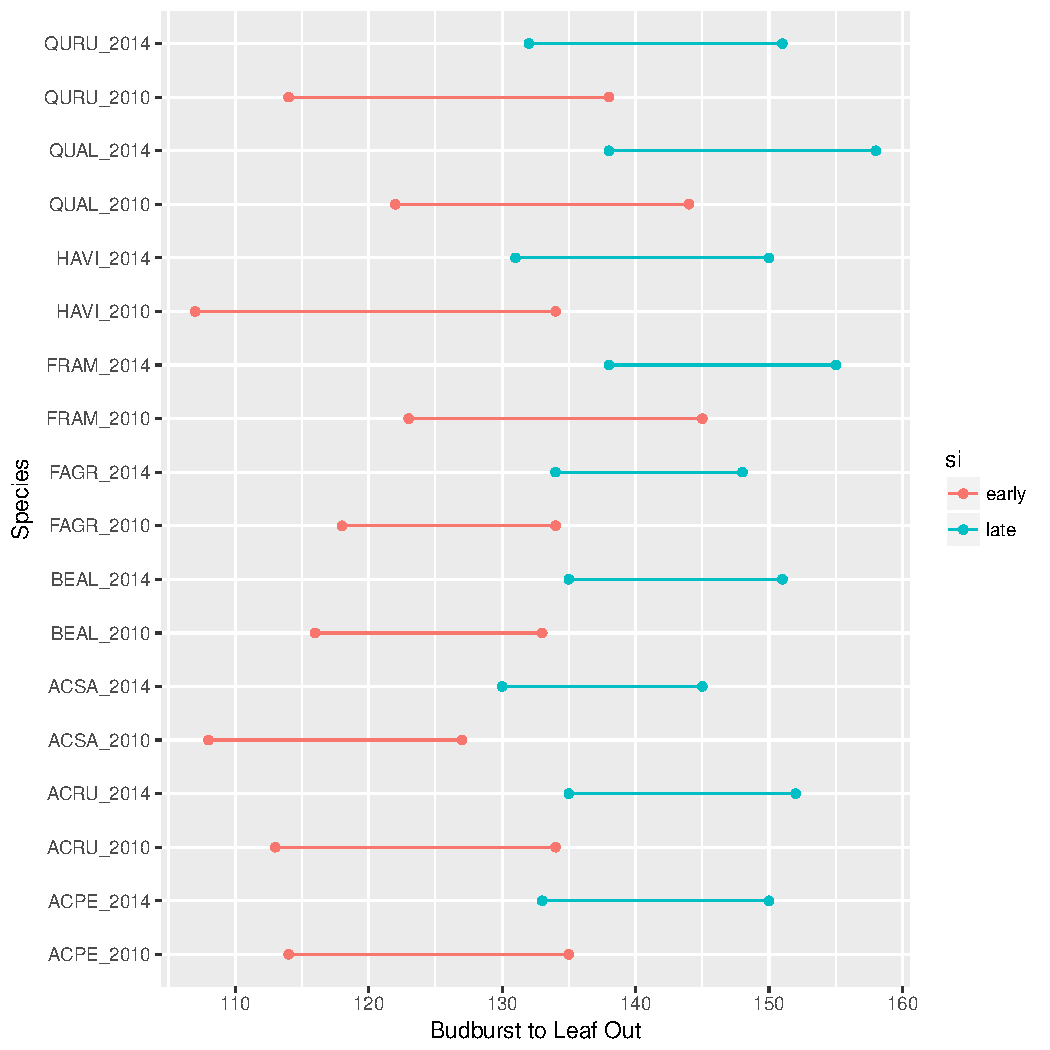
\includegraphics[width=\maxwidth]{figure/forest-1} \caption[A timeline plot indicating the duration of vegetative risk for each species from collected from Harvard Forest]{A timeline plot indicating the duration of vegetative risk for each species from collected from Harvard Forest.}\label{fig:forest}
\end{figure}




\section*{Regional Differences in Vegetative Risk?}
Lizzie: "Again need to build up for readers why regions might differ and how (basically get your readers to come up with your hypothesis before you spell it out) then 1) analyze lit for regional differences b) latitude analysis. And maybe a few other points you make here fit.

Based on this information, we analyzed two latitudinal gradients by downloading Daily Summary climate datasets from the NOAA Climate Data Online tool. We assessed 8-10 different degree latitude lines for each transect in order to measure frequency of false spring events \citep{Menne2012, Menne2012b}. False springs were tallied by first calculating the number of Growing Degree Days (GDD) with a base 10$^{\circ}$C temperature \citep{Nugent2005}.

If there were 40 GDDs before a hard freeze occurred in the spring (-2.2$^{\circ}$C), then it was determined that a false spring could have occurred in that year. Since we did not incorporate actual budburst or spring onset information, it is unclear whether these events were actually damaging. In order to simply address the climate question, we used these parameters to have a better understanding of the potential climate effects of latitude. 

Each location includes 30 years of climate data and each transect fell within 3 degrees longitude. Locations that were over 1,000m above sea level were excluded. 

\begin{figure} [H]
\begin{center}
\caption{Number of False Springs across two latitudinal gradients from 1986-2016: a) North American transect and b) European transect. More red dots have fewer false springs, whereas blue dots have more false springs. The size of the dot corresponds to frequency of false springs over the 30 year timeframe. }
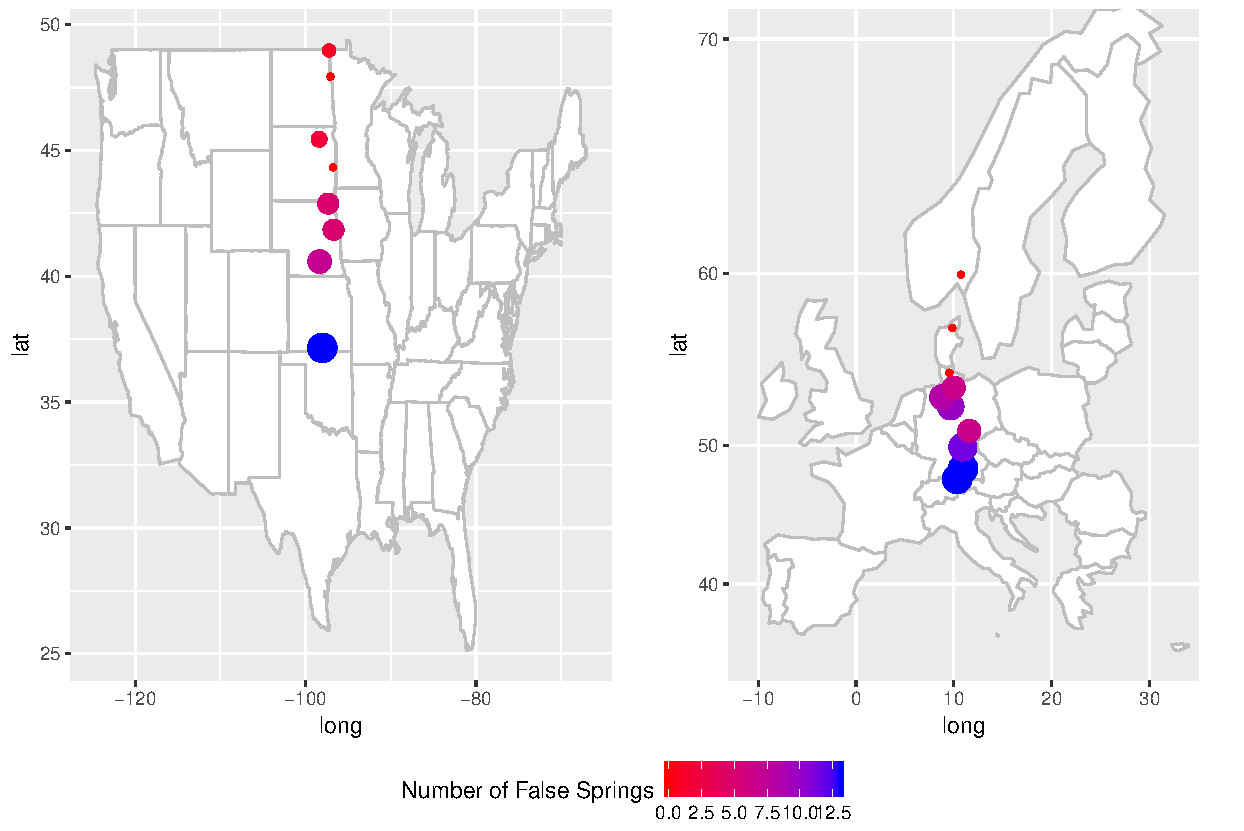
\includegraphics{..//figure/lat_maps.pdf}
\end{center}
\end{figure}

Table 4 shows the results from the linear regression models performed for both transects. Latitude (1) represents the European transect and Latitude (2) is the American transect. 


% Table created by stargazer v.5.2 by Marek Hlavac, Harvard University. E-mail: hlavac at fas.harvard.edu
% Date and time: Tue, Jan 24, 2017 - 10:22:39
\begin{table}[!htbp] \centering 
  \caption{The results from a linear regression model analyzing the relationship between latitude and frequency of false springs} 
  \label{} 
\begin{tabular}{@{\extracolsep{5pt}}lcc} 
\\[-1.8ex]\hline 
\hline \\[-1.8ex] 
 & \multicolumn{2}{c}{\textit{Dependent variable:}} \\ 
\cline{2-3} 
\\[-1.8ex] & \multicolumn{2}{c}{Latitude} \\ 
\\[-1.8ex] & (1) & (2)\\ 
\hline \\[-1.8ex] 
 False.Springs & $-$1.064$^{***}$ & $-$0.801$^{***}$ \\ 
  & (0.180) & (0.148) \\ 
  Constant & 57.235$^{***}$ & 46.946$^{***}$ \\ 
  & (0.936) & (0.865) \\ 
 \hline \\[-1.8ex] 
Observations & 10 & 8 \\ 
R$^{2}$ & 0.813 & 0.830 \\ 
Adjusted R$^{2}$ & 0.790 & 0.801 \\ 
Residual Std. Error & 1.743 (df = 8) & 1.732 (df = 6) \\ 
F Statistic & 34.885$^{***}$ (df = 1; 8) & 29.251$^{***}$ (df = 1; 6) \\ 
\hline 
\hline \\[-1.8ex] 
\textit{Note:}  & \multicolumn{2}{r}{$^{*}$p$<$0.1; $^{**}$p$<$0.05; $^{***}$p$<$0.01} \\ 
\end{tabular} 
\end{table} 


As seen in the above tables, as latitude increased the frequency of false spring events decreased. These results may indicate why species with a more northern range may have greater photoperiod sensitivities \citep{Caffarra2011} because the level of risk associated with a frost may in fact decrease. These findings demonstrate that further research needs to be pursued but they could ultimately indicate that certain latitudes should be prioritized for future false spring studies. 

\section*{Conclusion}

\section*{Supplemental}
Table 1 shows the results from the European transect investigated. False spring occurrence ranged from 0 to 8 and increased as latitude decreased. 

\begin{center}
\captionof{table}{Number of False Springs along a Latitudinal Gradient in Western Europe} \label{tab:title} 
\begin{tabular}{c c c c c}
\hline
Station & Elevation & Latitude & Longitude & False Springs \\
\hline
Kempten, Germany & 705m & 47.724 & 10.336 & 8 \\
Augsburg, Germany & 461m & 48.426 & 10.943 & 8 \\
Bamberg, Germany & 210m & 49.875 & 10.921 & 7 \\
Jena, Germany & 155m & 50.927 & 11.584 & 4 \\
Hannover, Germany & 55.0m & 52.466 & 9.679 & 6 \\
Bremen, Germany & 4.00m & 53.046 & 8.799 & 5 \\
Hamburg, Germany & 11.0m & 53.635 & 9.99 & 4 \\
Schleswig, Germany & 43.0m & 54.529 & 9.549 & 0 \\
Flyvestation, Denmark & 3.00m & 57.093 & 9.849 & 0 \\
Oslo, Norway & 94.0m & 59.943 & 10.721 & 0 \\
\hline
\end{tabular}
\end{center}

Table 2 shows the results from the American transect. False spring occurrence ranged from 0 to 13 and also exhibited an inverse relationship with latitude. 

\begin{center}
\captionof{table}{Number of False Springs along a Latitudinal Gradient in North America} \label{tab:title2} 
\begin{tabular}{c c c c c}
\hline
Station & Elevation & Latitude & Longitude & False Springs \\
\hline
Anthony, Kansas & 415m & 37.155 & -98.028 & 13 \\
Hastings, Nebraska & 587m & 40.583 & -98.350  & 7 \\
West Point, Nebraska & 399m & 41.845 & -96.714 & 5 \\
Yankton, South Dakota & 360m & 42.883 & -97.350 & 5 \\
Brookings, South Dakota & 497m & 44.325 & -96.769 & 0 \\
Aberdeen, South Dakota & 395m & 45.443 & -98.413 & 2 \\
Grand Forks, North Dakota & 253m & 47.933 & -97.083 & 0 \\
Pembina, North Dakota & 241m & 48.971 & -97.242 & 1 \\
\hline
\end{tabular}
\end{center}



\bibliography{..//refs/SpringFreeze.bib}
\end{document}
